\documentclass[10pt]{article}
\usepackage{graphicx}
\usepackage{amsmath}
\usepackage{float}
\usepackage{subcaption}
\usepackage[margin=1in]{geometry}


\begin{document}
\pagenumbering{gobble}
\begingroup  
  \centering
  \large Fast \& Sparse Learning with Compositional Concept Training\\[1em]
  \small{Andrew Lampinen* (lampinen@stanford.edu, Department of Psychology, Stanford University),\\ James McClelland (mclelland@stanford.edu, Department of Psychollogy, Stanford University)}\par
\endgroup
\vspace{10pt}
The end-to-end training on large data sets that is customary for neural networks is very unlike the way that adult humans learn tasks. Humans can learn rapidly from few examples. In part, this is likely because humans can be taught to break problems down into smaller parts, and can utilize previously learned concepts. Previous work has shown that to learn very difficult tasks in neural networks, it is sometimes necessary to teach intermediate steps of the task (G{\"{u}l\c{c}ehre \& Bengio, 2013). Here, we suggest that even if a task is easily learnable in general, the technique of teaching intermediate steps to the network can lead to much better performance on sparse data sets, and faster learning on larger data sets.\par
We demonstrate this by teaching networks the rules to Conway's Game of Life: For a square surrounded by eight neighboring squares, a square with four or more live neighbors dies from overcrowding, and one with fewer than two live neighbors dies of loneliness. A living square with two or three live neighbors lives, and a dead square with three live neighbors becomes alive. Calculating the life of a square under these rules can be decomposed into two separate steps: First, evaluating the current life of a unit and the number of its living neighbors, and second, computing its life at the subsequent time-step from these extracted features. This can be seen as a task of learning a mapping from 3 x 3 binary arrays (representing the current state) to a single binary value (representing the life of the central unit at the next time step). Since there are 512 possible input arrays, we trained on $n$ of them (randomly selected on each trial), and tested on the held out $512-n$, while varying $n$. We trained what we call a ``compositional'' network by training a single-layer (ReLU) network to extract number of neighbors and life of the central square from the input, and simultaneously training a single hidden-layer (tanh) network to compute the life value at the next time step from these extracted features. (We trained the second network off the output values produced by the first; training off the perfect values did not significantly alter the results.) We compared this compositional network to a variety of standard neural networks (one with two hidden layers, first ReLU, second tanh, to parallel the compositional, and then two networks with one of these hidden layers removed). These were trained to map the input directly to the output. (See Figure \ref{networkdiagram} for a comparison of our network to the two hidden layer standard network.) All training was done by SGD using MSE (learning rate=0.01, lr decay=0.99/epoch).\par
We demonstrated that the compositional network is able to learn from much sparser datasets than the standard networks. (See Figure \ref{n64figure} for a plot of error rate, averaged across 100 random training sets, each with $n = 64$ training examples. Note that the average error rates do not quite reach zero; even the compositional network was not always successful at learning the task with $n = 64$.) Furthermore, even with datasets sufficient for the standard networks to learn, the compositional network learned the task much more rapidly (see Figure \ref{n256figure}). We conclude that learning explicit compositions of subtasks can offer benefits for sparse learning, and for rapid learning even on large data sets, likely by constraining the solution space which must be searched. These training approaches may lead to more human-like learning from neural networks.
\vspace{-10pt}
\begin{figure}[H]
    \centering
    \begin{subfigure}[c]{0.35\textwidth}
	\centering
	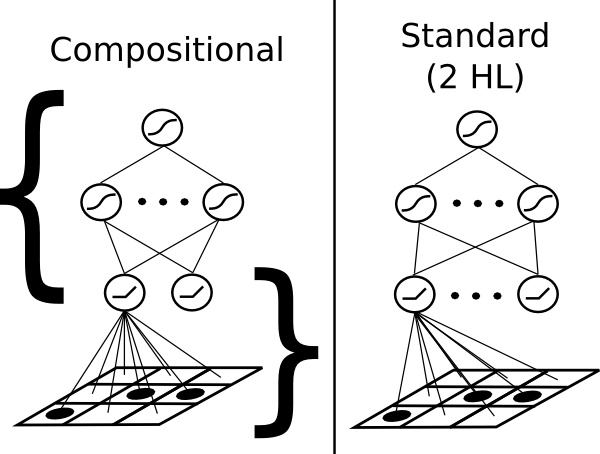
\includegraphics[width=\textwidth]{figures/hierarchical_NN_abstract_figure.png}
	\caption{Network comparison (brackets in compositional network denote the sub-networks we trained. All hidden layers had 10 units.)}
	\label{networkdiagram}
    \end{subfigure}
    \begin{subfigure}[c]{0.3\textwidth}
	\centering
	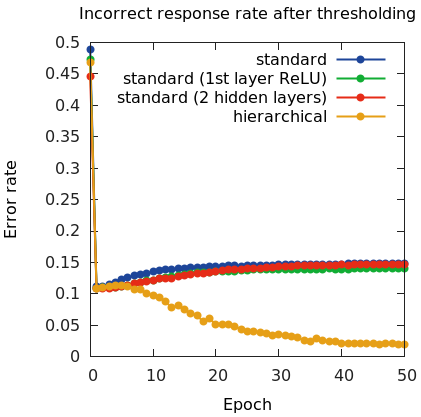
\includegraphics[width=\textwidth]{figures/n64figure.png}
	\caption{Error rates for $n = 64$}
	\label{n64figure}
    \end{subfigure}
    \begin{subfigure}[c]{0.3\textwidth}
	\centering
	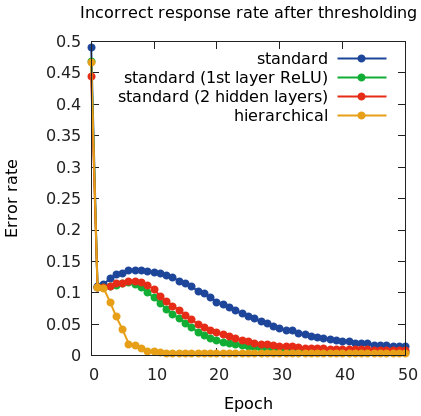
\includegraphics[width=\textwidth]{figures/n256figure.png}
	\caption{Error rates for $n = 256$}
	\label{n256figure}
    \end{subfigure}
    \caption{Network comparison \& results}
\end{figure}

\end{document}
